Mit diesem Experiment wird gezeigt, dass Agenten Ausweichbewegungen durchführen und Wartephasen einlegen, um andere Agenten passieren zu lassen.

\textbf{Aufbau des Experiments}
\begin{figure}[H]
    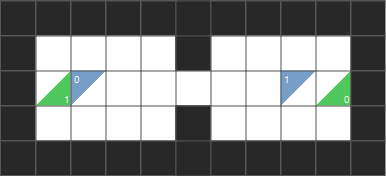
\includegraphics[height=40mm]{images/one_slit.png}
    \centering
    \caption{Aufbau für das Durchfahren zweier Agenten durch eine kurze Engstelle}
    \label{fig:engstelle}
\end{figure}
Die Karte misst neun mal drei Felder. In der Mitte der Karte ist eine eins mal eins Feld breite Engstelle. Auf beiden Seiten dieser Engstelle stehen sich Agenten gegenüber, die die Engstelle durchfahren müssen, um ihre Zielposition zu erreichen.

\textbf{Erwartete Beobachtungen}\newline
Der Agent, der zuerst einen Weg plant, fährt direkt auf seine Zielposition. Der andere Agent fährt eine Ausweichposition in der unmittelbaren Nähe der Engstelle an. Nachdem der erste Agent die Engstelle passiert hat, wird sich der zweite Agent auf direkten Weg zu seinem Ziel machen.